% LaTeX/Beamer preamble — pdflatex
% Generated by /course-maker course init. Edit freely.
% Engine-specific packages: fontenc + inputenc (required for pdflatex; remove if switching engines).

\documentclass[aspectratio=169, 10pt]{beamer}

% ── Theme ───────────────────────────────────────────────────────────────────
\usetheme{Madrid}
\usecolortheme{default}
\setbeamertemplate{navigation symbols}{}
\setbeamertemplate{footline}[frame number]

% ── Packages ────────────────────────────────────────────────────────────────
\usepackage[T1]{fontenc}
\usepackage[utf8]{inputenc}
\usepackage[english]{babel}   % replace with course language: russian, french, german, etc.
\usepackage{amsmath, amssymb, amsfonts}
\usepackage{graphicx}
\usepackage{booktabs}
\usepackage{tikz}
\usetikzlibrary{arrows.meta, positioning, shapes.geometric}
\usepackage{xcolor}

% ── Colors ──────────────────────────────────────────────────────────────────
\definecolor{mainblue}{RGB}{46,64,87}
\definecolor{accent}{RGB}{232,72,85}

% ── Title info ──────────────────────────────────────────────────────────────
\title{Regularization in Machine Learning}
\subtitle{Lecture 1. Regularization Foundations}
\author{Sonnet 5 High}
\institute{Claude Cowork}
\date{\today}

\begin{document}

% Slide 01 — Title slide
\begin{frame}
  \titlepage
\end{frame}

% Slide 02 — Outline
\begin{frame}{Outline}
  \begin{itemize}
    \item Why models overfit \& the bias--variance tradeoff
    \item Ridge and Lasso: mechanics and geometry
    \item Choosing $\lambda$ and the Bayesian view
    \item Elastic net teaser \& wrap-up
  \end{itemize}
\end{frame}

% Slide 03 — Why do models overfit?
\begin{frame}{Why do models overfit?}
  More parameters give a model more capacity to fit the training data --- including its noise, not just the underlying pattern.
  \begin{center}
    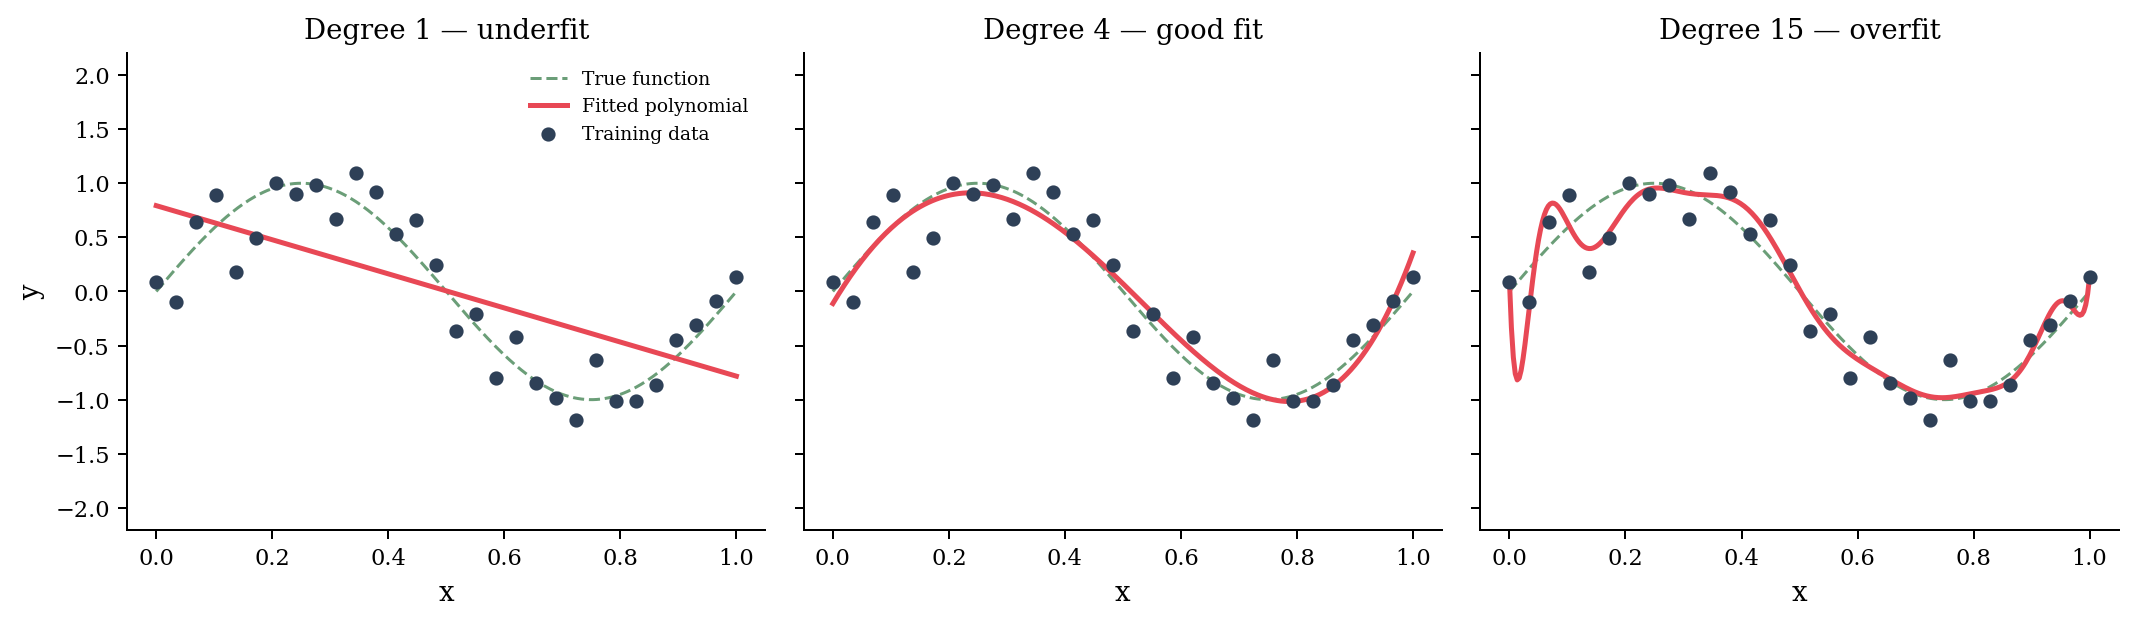
\includegraphics[width=\textwidth, height=0.55\textheight, keepaspectratio]{figures/fig01_polynomial_fits.png}
  \end{center}
\end{frame}

% Slide 04 — The bias-variance tradeoff
\begin{frame}{The bias-variance tradeoff}
  Expected test error decomposes into three additive terms:
  \[
    \mathbb{E}\big[(y - \hat{f}(x))^2\big] \;=\; \underbrace{\text{Bias}[\hat f(x)]^2}_{\text{model too simple}} \;+\; \underbrace{\text{Var}[\hat f(x)]}_{\text{sensitive to training sample}} \;+\; \underbrace{\sigma^2}_{\text{irreducible noise}}
  \]
  \begin{itemize}
    \item \textbf{Bias:} systematic error from a model that can't capture the true pattern
    \item \textbf{Variance:} how much the fitted model changes across different training samples
    \item Regularization trades a small increase in bias for a larger reduction in variance
  \end{itemize}
\end{frame}

% Slide 05 — Overfitting in numbers
\begin{frame}{Overfitting in numbers}
  \begin{columns}[c]
    \begin{column}{0.48\textwidth}
      \begin{itemize}
        \item Training error keeps falling as complexity grows
        \item Validation error is U-shaped --- it eventually rises
        \item The growing gap between the two curves is the signature of overfitting
      \end{itemize}
    \end{column}
    \begin{column}{0.48\textwidth}
      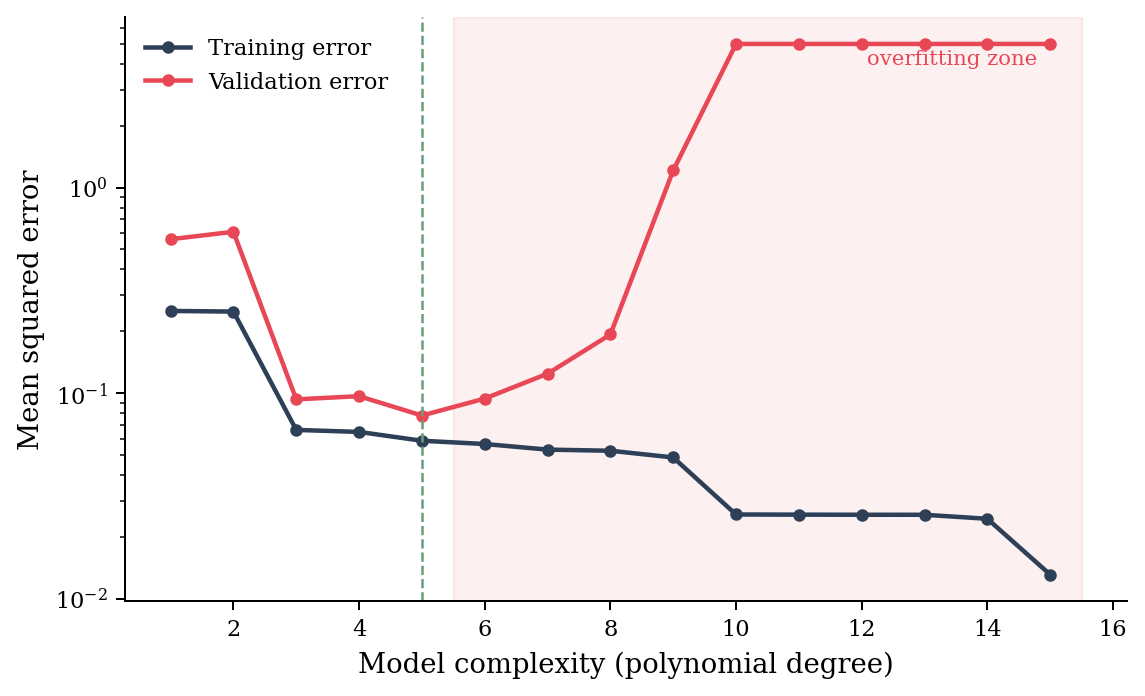
\includegraphics[width=\textwidth, height=0.55\textheight, keepaspectratio]{figures/fig02_train_val_error.png}
    \end{column}
  \end{columns}
\end{frame}

% Slide 06 — What is regularization?
\begin{frame}{What is regularization?}
  \begin{block}{Definition}
    Any technique that discourages a model from fitting the training data too closely, without changing the model family --- typically by adding a penalty or constraint tied to model complexity.
  \end{block}
  \begin{itemize}
    \item Alternative: manually pick a simpler model (fewer features) --- crude and inflexible
    \item Regularization lets a tunable strength decide how much complexity the data actually supports
  \end{itemize}
\end{frame}

% Slide 07 — Ridge regression: the L2 penalty
\begin{frame}{Ridge regression: the L2 penalty}
  \[
    \hat\beta_{\text{ridge}} = \arg\min_\beta \; \underbrace{\|y - X\beta\|_2^2}_{\text{fit to data}} \;+\; \lambda \underbrace{\|\beta\|_2^2}_{\text{penalty}}
  \]
  \begin{itemize}
    \item $\lambda = 0$: recovers ordinary least squares exactly
    \item $\lambda \to \infty$: all coefficients pushed toward zero
    \item The intercept is conventionally left out of the penalty
  \end{itemize}
\end{frame}

% Slide 08 — Ridge: effect on coefficients
\begin{frame}{Ridge: effect on coefficients}
  \begin{columns}[c]
    \begin{column}{0.48\textwidth}
      \begin{itemize}
        \item As $\lambda$ grows, every coefficient shrinks smoothly toward zero
        \item Coefficients essentially never land exactly on zero
        \item Ridge keeps all features, just with smaller weight
      \end{itemize}
    \end{column}
    \begin{column}{0.48\textwidth}
      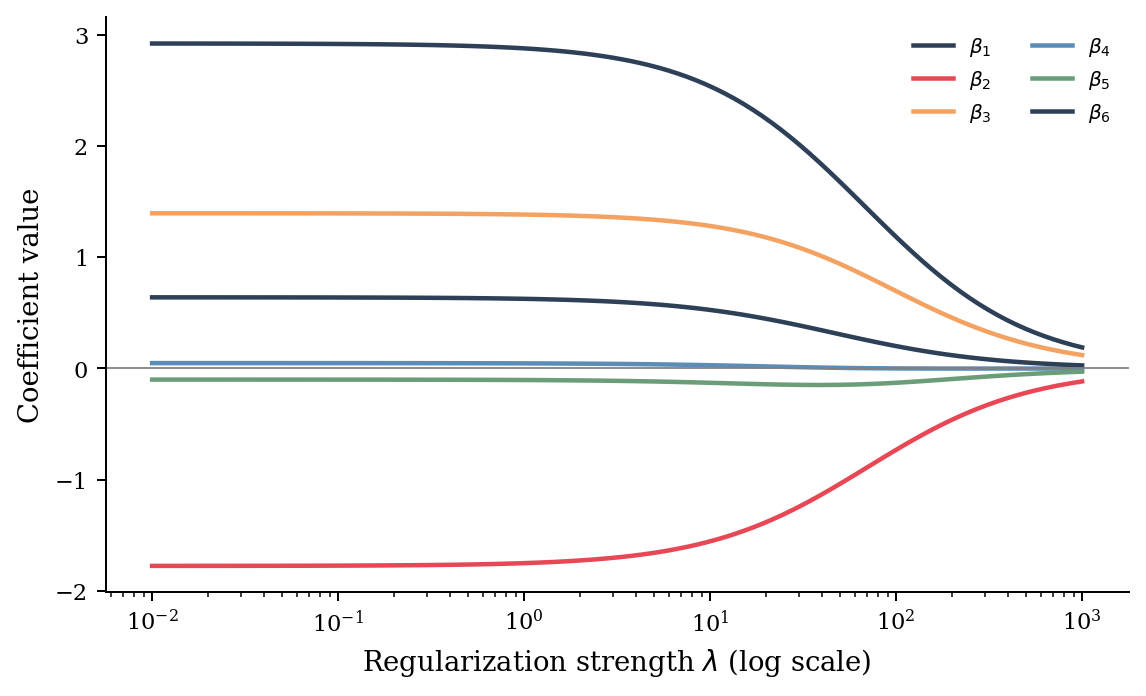
\includegraphics[width=\textwidth, height=0.55\textheight, keepaspectratio]{figures/fig03_ridge_shrinkage.png}
    \end{column}
  \end{columns}
\end{frame}

% Slide 09 — Geometric picture: L2
\begin{frame}{Geometric picture: L2}
  \begin{columns}[c]
    \begin{column}{0.46\textwidth}
      \begin{itemize}
        \item Ridge is exactly equivalent to minimizing the loss subject to $\|\beta\|_2 \le t$
        \item The solution sits where the smallest loss contour touches the circular boundary
        \item A circle has no corners --- the tangency point generically has both coordinates nonzero
      \end{itemize}
    \end{column}
    \begin{column}{0.5\textwidth}
      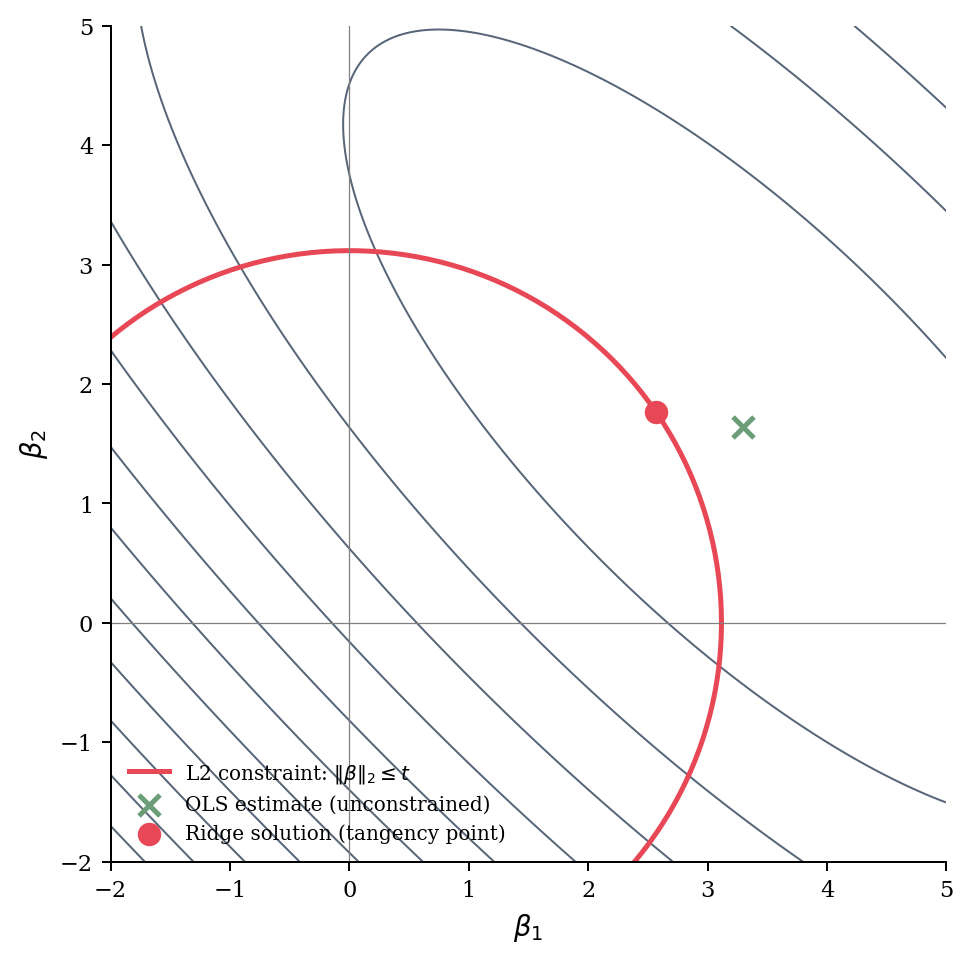
\includegraphics[width=\textwidth, height=0.55\textheight, keepaspectratio]{figures/fig04_l2_geometry.png}
    \end{column}
  \end{columns}
\end{frame}

% Slide 10 — Lasso regression: the L1 penalty
\begin{frame}{Lasso regression: the L1 penalty}
  \[
    \hat\beta_{\text{lasso}} = \arg\min_\beta \; \underbrace{\|y - X\beta\|_2^2}_{\text{fit to data}} \;+\; \lambda \underbrace{\|\beta\|_1}_{\text{penalty}}
  \]
  \begin{itemize}
    \item Same idea as ridge --- penalize the loss --- with a different norm
    \item $\|\beta\|_1 = \sum_j |\beta_j|$, the sum of absolute values
    \item Unlike the L2 penalty, this norm can push coefficients to exactly zero
  \end{itemize}
\end{frame}

% Slide 11 — Geometric picture: L1 and sparsity
\begin{frame}{Geometric picture: L1 and sparsity}
  \begin{columns}[c]
    \begin{column}{0.46\textwidth}
      \begin{itemize}
        \item Lasso is equivalent to minimizing the loss subject to $\|\beta\|_1 \le t$ --- a diamond-shaped region
        \item The loss contour typically first touches the diamond at a corner
        \item At a corner, one coordinate is exactly zero --- lasso performs automatic feature selection
      \end{itemize}
    \end{column}
    \begin{column}{0.5\textwidth}
      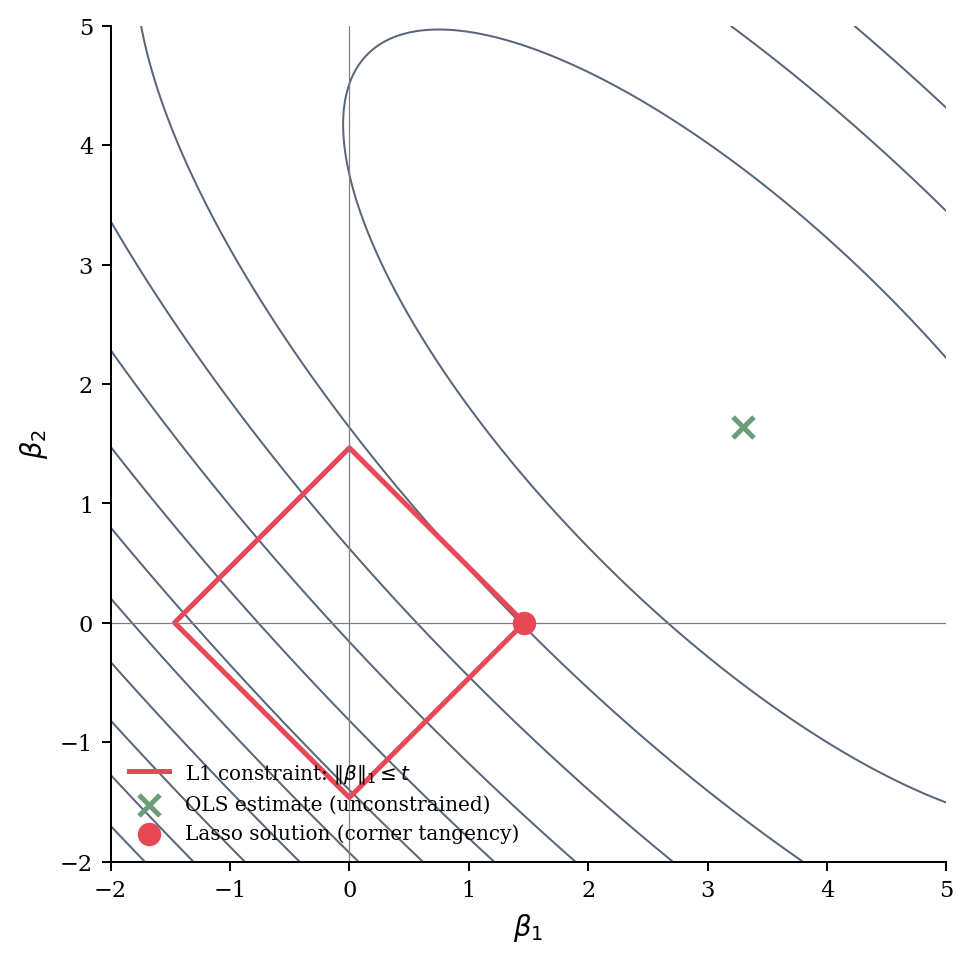
\includegraphics[width=\textwidth, height=0.55\textheight, keepaspectratio]{figures/fig05_l1_geometry.png}
    \end{column}
  \end{columns}
\end{frame}

% Slide 12 — Ridge vs. Lasso
\begin{frame}{Ridge vs. Lasso}
  \begin{center}
  \small
  \begin{tabular}{lll}
    \toprule
    & \textbf{Ridge (L2)} & \textbf{Lasso (L1)} \\
    \midrule
    Sparsity & No & Yes \\
    Correlated features & Shrinks together & Picks one, zeros others \\
    Solution & Always unique & May not be unique \\
    Computation & Closed form & Iterative (e.g.\ coordinate descent) \\
    \bottomrule
  \end{tabular}
  \end{center}
  \vspace{0.5em}
  Rule of thumb: use lasso when you suspect many irrelevant features; use ridge when most features carry some signal.
\end{frame}

% Slide 13 — Choosing the regularization strength lambda
\begin{frame}{Choosing the regularization strength $\lambda$}
  $\lambda$ is a hyperparameter --- it is chosen by evaluating held-out performance across a grid of values via cross-validation, not learned from the training objective directly.
  \begin{center}
    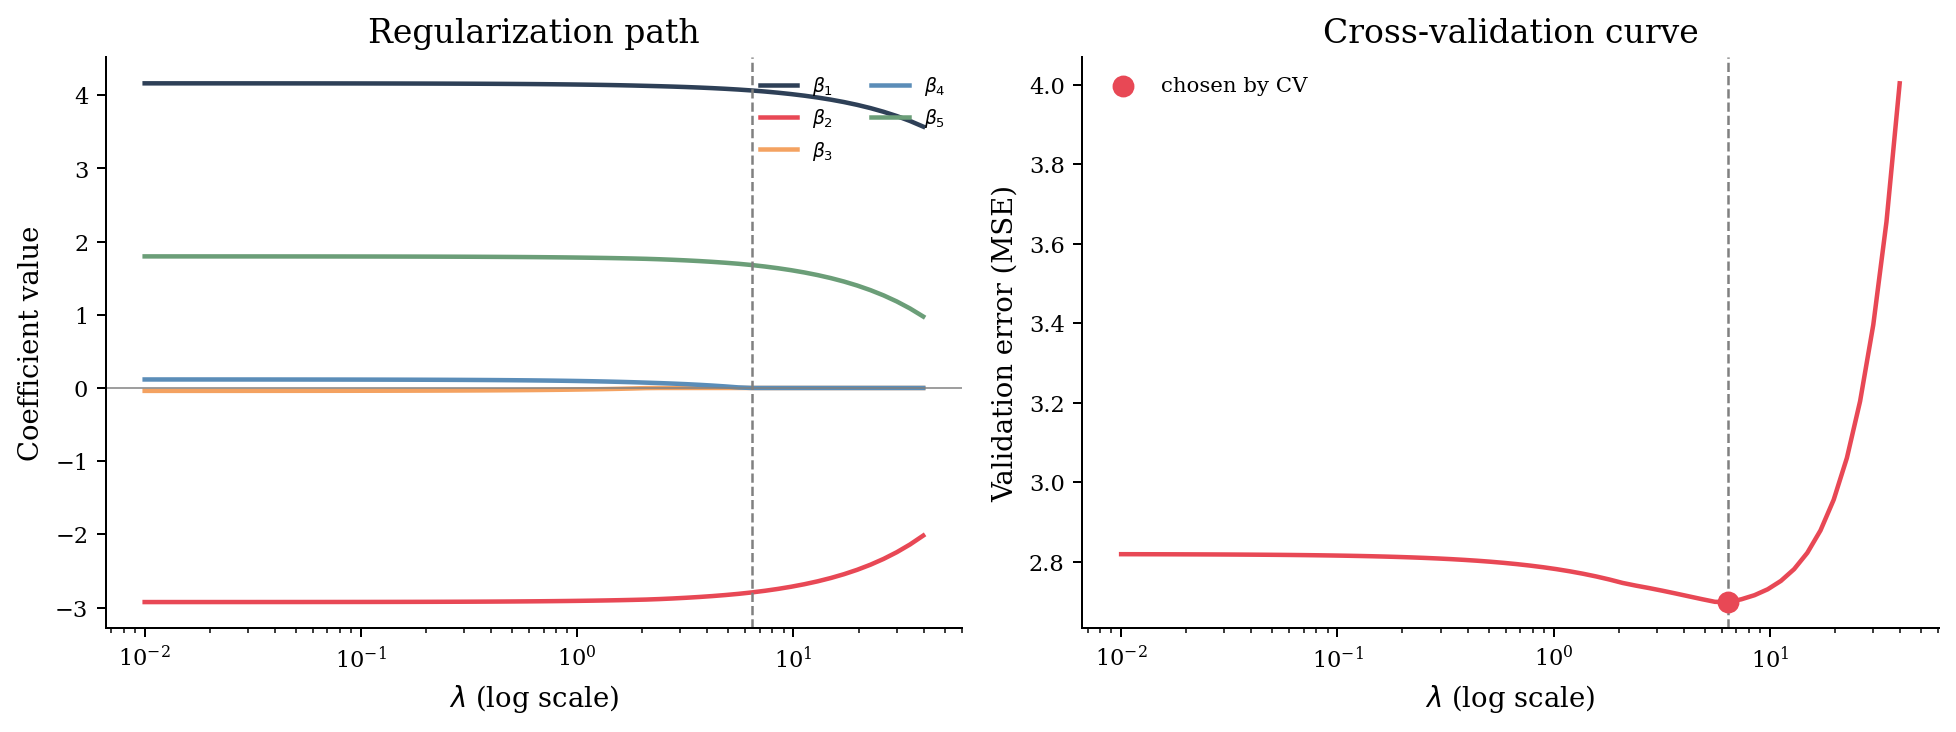
\includegraphics[width=\textwidth, height=0.5\textheight, keepaspectratio]{figures/fig06_lasso_path_cv.png}
  \end{center}
\end{frame}

% Slide 14 — Regularization as prior belief
\begin{frame}{Regularization as prior belief}
  \begin{block}{Key idea}
    Adding a penalty term to the loss is mathematically equivalent to placing a prior distribution over the parameters and computing the maximum a posteriori (MAP) estimate.
  \end{block}
  \begin{itemize}
    \item ``Penalty strength'' becomes ``how strongly we believe, before seeing data, that coefficients should be small''
    \item This reframes ridge and lasso as different \emph{prior beliefs} about the coefficients
  \end{itemize}
\end{frame}

% Slide 15 — MAP interpretation: Ridge <-> Gaussian prior
\begin{frame}{MAP interpretation: Ridge $\leftrightarrow$ Gaussian prior}
  Assume each coefficient has an independent prior $\beta_j \sim \mathcal{N}(0, \tau^2)$. The MAP estimate maximizes the posterior, equivalent to minimizing:
  \[
    -\log p(y \mid X, \beta) - \log p(\beta) \;=\; \underbrace{\|y - X\beta\|_2^2}_{\text{data term}} \;+\; \underbrace{\frac{\sigma^2}{\tau^2} \|\beta\|_2^2}_{\text{= ridge penalty}} \;+\; \text{const}
  \]
  \begin{itemize}
    \item The Gaussian prior is symmetric and ``soft'' around zero
    \item This is exactly why ridge shrinks smoothly rather than zeroing out coefficients
  \end{itemize}
\end{frame}

% Slide 16 — MAP interpretation: Lasso <-> Laplace prior
\begin{frame}{MAP interpretation: Lasso $\leftrightarrow$ Laplace prior}
  Assume each coefficient has an independent prior $\beta_j \sim \text{Laplace}(0, b)$. The MAP estimate is equivalent to minimizing:
  \[
    -\log p(y \mid X, \beta) - \log p(\beta) \;=\; \underbrace{\|y - X\beta\|_2^2}_{\text{data term}} \;+\; \underbrace{\frac{2\sigma^2}{b} \|\beta\|_1}_{\text{= lasso penalty}} \;+\; \text{const}
  \]
  \begin{itemize}
    \item The Laplace prior has a sharp peak at zero
    \item This is the probabilistic reason lasso favors exact zeros --- the same conclusion as the geometric picture, from a different angle
  \end{itemize}
\end{frame}

% Slide 17 — Putting it together
\begin{frame}{Putting it together}
  Three equivalent ways to understand regularization:
  \begin{itemize}
    \item \textbf{Bias-variance:} controls model complexity to reduce variance
    \item \textbf{Geometric:} constrains coefficients to a norm ball (circle vs.\ diamond)
    \item \textbf{Bayesian:} encodes a prior belief that coefficients should be small (Gaussian vs.\ Laplace)
  \end{itemize}
  All three give the same answer --- keep whichever lens is most intuitive.
\end{frame}

% Slide 18 — Beyond L1/L2: elastic net (announce only)
\begin{frame}{Beyond L1/L2: elastic net}
  \begin{itemize}
    \item Combining both penalties gets some of lasso's sparsity together with ridge's stability under correlated features
    \item Objective: $\|y - X\beta\|_2^2 + \lambda_1 \|\beta\|_1 + \lambda_2 \|\beta\|_2^2$
    \item A single blend parameter interpolates between pure ridge and pure lasso
  \end{itemize}
\end{frame}

% Slide 19 — Summary & closing
\begin{frame}{Summary \& closing}
  \begin{itemize}
    \item Overfitting is a complexity problem: models with too much capacity memorize noise, not signal
    \item Ridge (L2) and lasso (L1) are the two foundational tools --- shrinkage vs.\ shrinkage + selection
    \item Both have equivalent readings as constrained optimization and as Bayesian priors
    \item $\lambda$ is chosen by cross-validation, not guessed
  \end{itemize}
  \vspace{0.5em}
  Next lecture: elastic net and regularization for deep learning, then we put it all into practice in the lab.
\end{frame}

\end{document}

